\documentclass[svgnames,14pt]{beamer}
\usepackage{caption}
\usepackage{graphicx}
\usepackage{xcolor}
\title{Genomes Comparision via de Bruijn graphs}
\author{Student: Ilya Minkin \\ Advisor: Son Pham}
\institute{St. Petersburg Academic University}
\setbeamertemplate{footline}[frame number]
\setbeamertemplate{navigation symbols}{}
\setbeamertemplate{caption}[numbered]
\begin{document}
\maketitle

\begin{frame}
\frametitle{Biological Motivation}
\begin{itemize}
\item  Sequencing genomes is getting cheaper 
\item Probably genome assembly task will be easier with current development in sequencing machines (Nanopore) 
    \begin{itemize}
    \item  1000 Human Genomes
    \item Genomes 10K: One genome for each vetebrate genus
    \item 1001  Arabidopsis Genomes
    \item Human Microbiome Project: sequence genomes of microbial communities at different sites on human body
    \end{itemize}
\item  What can we do with these \textbf{thousands} of sequences?
\end{itemize}

\end{frame}

\begin{frame}
\frametitle{Long Term Project}

\begin{itemize}
\item None of the current comparative genomics tools were designed for a very high number of genomes.
\item We aim to  provide a tool for comparing multiple genomes that has the following functions (properties)
\begin{itemize}
\item Find synteny blocks in (multiple) complicated genomes
\item Allocate insertions, deletions
\item Find other structure variations
\item Ability to work for incomplete genomes (contigs)
\item Provide a user friendly web interface for this tool.
\end{itemize}
\end{itemize}
\end{frame}

\begin{frame}
\frametitle{Synteny Blocks: Algorithmic challenge}
\begin{itemize}
\item Suppose that we are given two genomes
\item The question is: how are they evolutionary related to each other?
\item In order to do rearrangements analysis we must decompose genomes into synteny blocks
\item Synteny blocks are evolutionary conserved segments of the genome
\item These blocks cover most of the genome
\item Occur in both genomes with possible variations
\end{itemize}
\end{frame}

\begin{frame}
\frametitle{Academic Project}

Project: Identify synteny blocks for duplicated genomes represented as sequences of \textbf{nucleotides}.

\begin{itemize}
\item \textbf{None} of the previous synteny blocks reconstruction software (DRIMM-Synteny (Pham And Pevzner 2010) included) can 
efficiently solve this problem. 
\item DRIMM-Synteny can find the synteny blocks for complicated genomes. But:
\pause \item It requires the genome to be represented as sequence of genes. 
\end{itemize}
%\pause
%Challenge: <-- I think that this should be introduced later, after de Bruijn graphs and etc (Ilya)
%\begin{itemize}
%\item Double strands
%\item Graph Simplification for double strands.
%\item Memory efficient.
%\end{itemize}
\end{frame}

%\begin{frame}
%\frametitle{Example}
%\begin{figure}
%\centering
%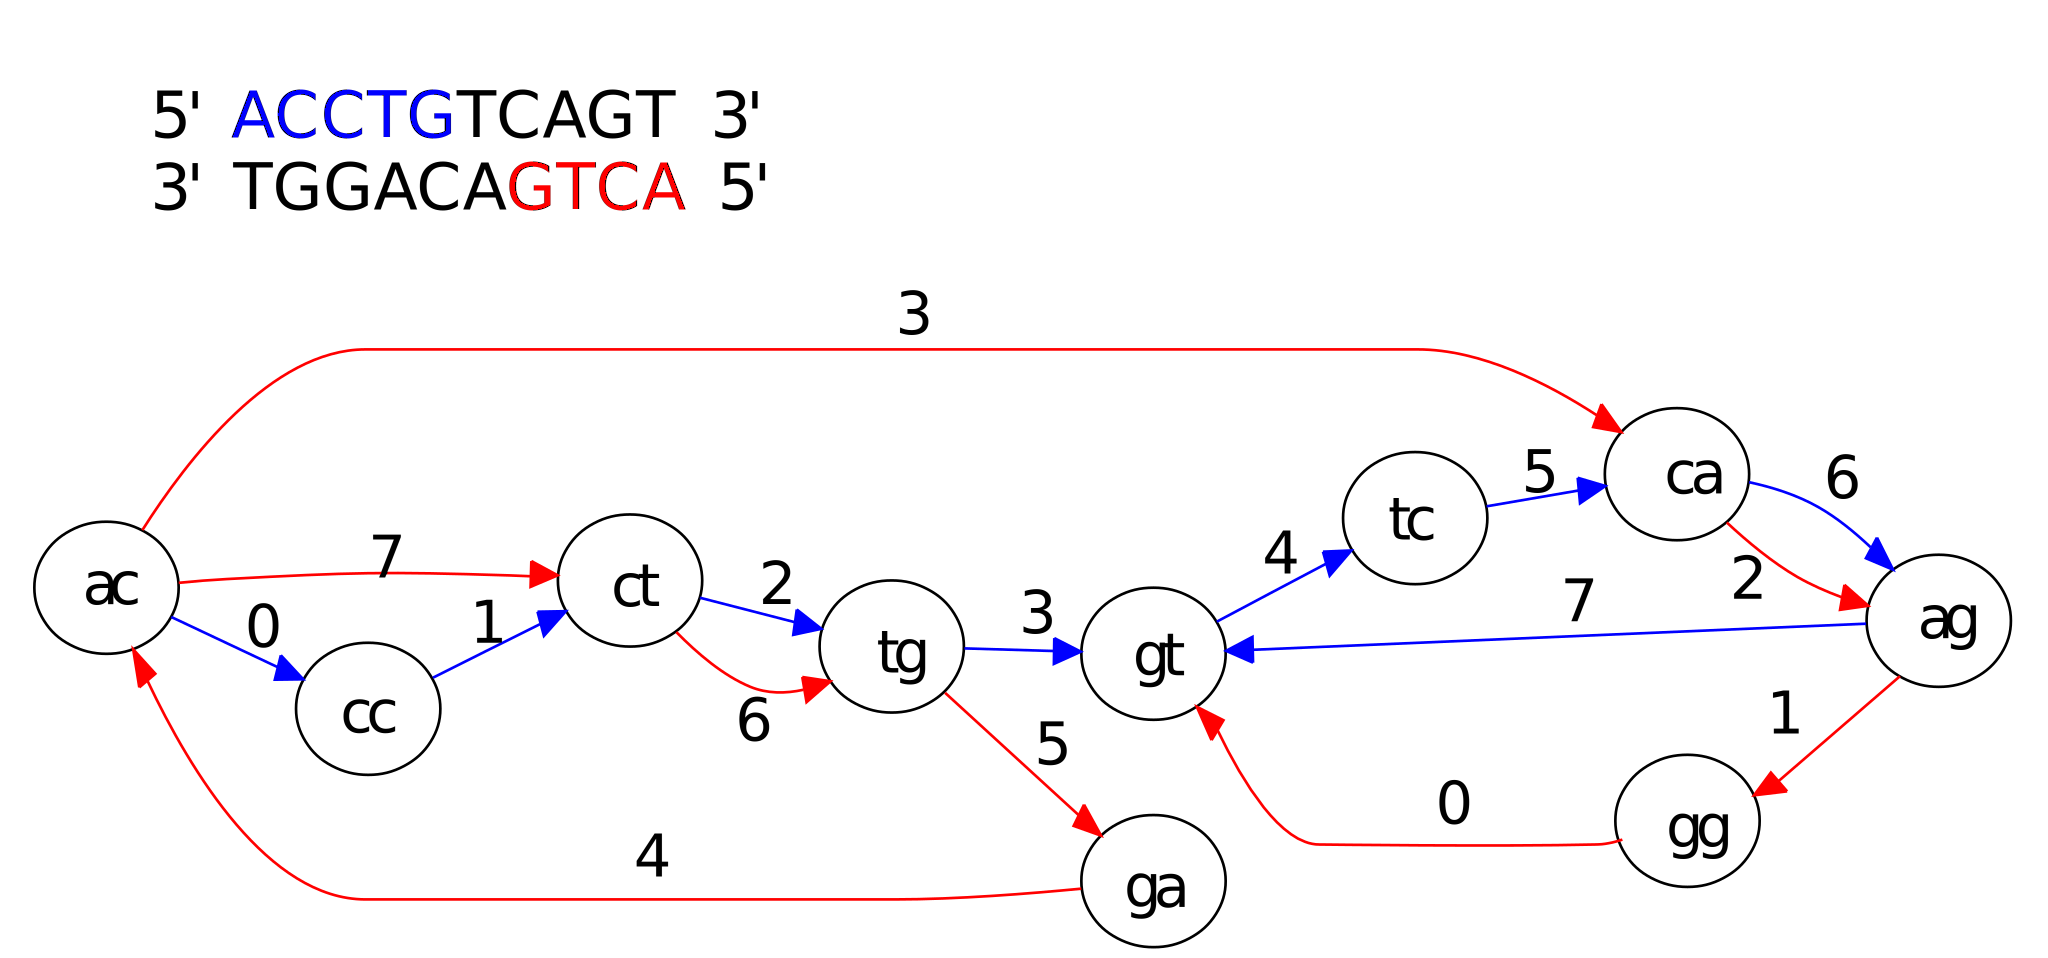
\includegraphics[scale = 0.40]{Figure1.pdf}
%\small \caption{Possible transformation of the mouse X chromosome into the human one [Pevzner, Tesler 2003]. Each synteny block (numbered box) corresponds to a genome region.}
%\end{figure}
%\end{frame}

%\begin{frame}
%\frametitle{A typical algorithm}
%\begin{itemize}
%\item Place genomes along the axes of the 2-D dot plot
%\pause \item Represent each anchor as a dot on the plot
%\pause \item Glue together anchors that form diagonals
%\pause \item Project each diagonal on the corresponding axis
%\begin{figure}
%\centering
%\includegraphics[scale = 0.40]{Figure2.pdf}
%\small \caption{Illustration of working of an algorithm (GRIMM) [Pham, Pevzner 2010]}
%\end{figure}
%\end{itemize}
%\end{frame}

%\begin{frame}
%\frametitle{The problem}
%\begin{itemize}
%\item If the genomes are highly duplicated, diagonals will overlap
%\pause \item The result is the ovelapping synteny blocks
%\pause \item We want non-overlapping blocks
%\pause \item New approach - build de Bruijn graph over the nucleotides
%\pause \item No anchors
%\end{itemize}
%\end{frame}

\begin{frame}
\frametitle{General Idea: de Bruijn Graph}
\begin{itemize}
\item Create de Bruijn graph from the nucleotide sequence - no anchors
\item Conserved regions will yield non-branching paths
\item We are given an alphabet \( \Sigma \) and a string \( S \) over it, \(|\Sigma| = m \)
\item A substring \( T, \, |T| = k \) is called \textit{k-mer}
\item de Bruijn graph is a multigraph \( G_{k} = (V, E) \), where \\
\( V = \Sigma^{k - 1} = \) \{all possible strings of length k-1\} \\
\item If \(k\)-mer \( T \) is present in \( S \) then we add oriented edge \( (T[1, k - 1], T[2, k]) \) to the graph
\end{itemize}
\end{frame}

\begin{frame}
\frametitle{Challenges}
\begin{itemize}
\item Variations in synteny blocks generate cycles, so we need to simplify graph
\item Double strandness: conserved regions may occur on both strands. Example: \\
5' \textcolor{Green}{AACC}GGTT 3' \\
3' TTGG\textcolor{Green}{CCAA} 5'
\item Such blocks are reversed complementary to each other \( \Rightarrow \) no non-branching paths
\item Memory efficiency
\end{itemize}
\end{frame}

\begin{frame}
\frametitle{First Example: Ideal Situation}
\begin{figure}
\centering
\includegraphics[scale = 0.60]{Figure3.pdf}
\small \caption{Here absolutely conserved region "ACGTG" generates clear non-branching path}
\end{figure}
\end{frame}

\begin{frame}
\frametitle{Second Example: SNP}
\begin{figure}
\centering
\includegraphics[scale = 0.60]{Figure4.pdf}
\small \caption{In this example SNP generates so-called "bulge" cycle}
\end{figure}
\end{frame}

\begin{frame}
\frametitle{Double Strands: Possible Solutions}
\begin{itemize}
\item Colored de Bruijn graph. Build two graphs for the direct and the reverse-complementary sequences. Color edges in each graph and merge graphs
\item Bidirected graph. Each vertex has two parts -- direct and reverse complementary. Every edge has two directions (one on each end) to indicate which part of the vertex we use
\item Simplest possible solution -- glue \( k \)-mers that are reverse complementary
\end{itemize}
\end{frame}

\begin{frame}
\frametitle{Third Example: Double Strands}
\begin{figure}
\centering
\includegraphics[scale = 0.60]{Figure5.pdf}
\small \caption{Gluing reverse complementary edges helps to resolve double strandness issue}
\end{figure}
\end{frame}

\begin{frame}
\frametitle{Methods and expected results}
\begin{itemize}
\item Glue complementary \(k\)-mers togetther
\item Simplify graph by deleting short cycles \\ (with size less than some \( \Delta \))
\item Note that our graph simplification is different from the graph simplification in genome assemblers
\item Find non branching paths = synteny blocks
\item Use the software to analyse repeats in Arabidopsis genome
%\pause \item Collaborate with some cool guys from SALK institute <-- This should be in caution since we do not have any results YET.
\end{itemize}
\end{frame}

\begin{frame}
\frametitle{Current Progress}
Now:
\begin{itemize}
\item Program that can find absolutely conserved regions on one strand
\item Handles 25 MB Arabidopsis chromosome \\ with  \( \le \) 500 MB RAM
\end{itemize}
Near future:
\begin{itemize}
\item Add graph simplification
\item Resolve double strandness issue
\item Get rid of hashtables, use suffix arrays \( \Rightarrow \) reduced memory consumption
\end{itemize}
\end{frame}

\begin{frame}
\frametitle{References}
\begin{itemize}
\item 1. Pevzner P and Tesler G, (2003) Human and mouse genomic sequences reveal extensive breakpoint reuse in mammalian evolution. 
\item 2. Pham S and Pevzner P, (2010) DRIMM-Synteny: Decomposing Genomes into Evolutionary Conserved Segments
\end{itemize}
\end{frame}

\begin{center}
\hfill \huge \\
\vspace{60pt}
Thank you!
\end{center}

\end{document}
